\section{第一章测试题}

\begin{enumerate}

\item 设
$P=\left\{x \mid (x+1)^2\le 4,\ \text{且}\ x\in \mathbb{R}\right\},\quad
Q=\left\{x \mid 5\le x^2+16,\ \text{且}\ x\in \mathbb{R}\right\},$
则下列命题正确的是\underline{\hspace{2cm}}.

\begin{choices}
	\item $Q\subseteq P$
	\item $Q\subset P$
	\item $P=Q$
	\item $P\subset Q$
\end{choices}

\item 设 \(A=\{a,\{a\}\}\),下列命题错误的是(\quad).
\begin{choices}
	\item \(\{a\}\in P(A)\)
	\item \(\{\{a\}\}\in P(A)\)
	\item \(\{a\}\subseteq P(A)\)
	\item \(\{\{a\}\}\subseteq P(A)\)
\end{choices}

\item 在 $0(\ \ )\varnothing$ 之间写上正确的符号.
\begin{choices}
	\item $\subseteq$
	\item $\in$
	\item $=$
	\item $\notin$
\end{choices}

\item 若 $A-B=\Phi$,则下列哪个结论不可能正确(\quad).
\begin{choices}
	\item $A\subset B$
	\item $A=\Phi$
	\item $B\subset A$
	\item $B=\Phi$
\end{choices}

\item 判断下列哪个命题为真(\quad).
\begin{choices}
	\item 空集只是非空集合的子集
	\item 若 $A$ 的一个元素属于 $B$,则 $A=B$
	\item $A-B=B-A \Rightarrow A=B$
	\item 空集是任何集合的真子集
\end{choices}

\item 设$\{a,b,c\},\ *$为代数系统,$*$运算如下:
\begin{table}[H]
	\centering
	\begin{tabular}{|c|c|c|c|}
		\hline
		$*$ & $a$ & $b$ & $c$ \\
		\hline
		$a$ & $a$ & $b$ & $c$ \\
		\hline
		$b$ & $b$ & $a$ & $c$ \\
		\hline
		$c$ & $c$ & $c$ & $c$ \\
		\hline
	\end{tabular}
\end{table}

则零元为(\qquad).
\begin{choices}
	\item 没有
	\item $b$
	\item $a$
	\item $c$
\end{choices}

\item N 是自然数集,定义\(f:\mathbb{N}\to\mathbb{N}\),\(f(x)=x \bmod 3\)(即 \(x\) 除以 \(3\) 的余数),则 \(f\) 是(\hspace{2em}).
\begin{choices}
	\item 满射不是单射
	\item 双射
	\item 单射不是满射
	\item 不是单射也不是满射
\end{choices}

\item 下面函数(\quad)是单射而非满射.
\begin{choices}
	\item $f:\mathbb{R}\to\mathbb{R},\quad f(x)=2x+1$
	\item $f:\mathbb{R}\to\mathbb{Z},\quad f(x)=\lfloor x\rfloor$,$\lfloor x\rfloor$ 表示不大于 $x$ 的最大整数
	\item $f:\mathbb{R}\to\mathbb{R},\quad f(x)=-x^2+2x-1$
	\item $f:\mathbb{Z}^{+}\to\mathbb{R},\quad f(x)=\ln x$
\end{choices}
	
\item 若 $S=\{S_1,S_2,\cdots,S_m\}$ 是集合 $A$ 的一个分划,则它应满足条件\underline{\hspace{2cm}}.


\item 设$A = \left\{\langle 1,2\rangle,\langle 2,4\rangle,\langle 3,3\rangle\right\},\quad B = \left\{\langle 1,3\rangle,\langle 2,4\rangle,\langle 4,2\rangle\right\}.$ 

则$A \cup B = \underline{\hspace{2cm}}.\quad A \circ B = \underline{\hspace{2cm}}.$


\item 若集合 $S$ 的基数 $|S|=5$,则 $S$ 的幂集的基数 $|P(S)|=\underline{\hspace{2cm}}$.


\item A,B,C表示三个集合,文氏图中阴影部分的集合表达式为$\underline{\hspace{2cm}}$.

\begin{figure}[H]
	\centering
	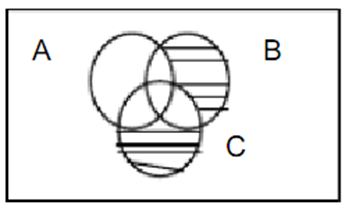
\includegraphics[width=0.2\linewidth]{figure/1-2-4}
	\caption{习题1-2-4图}
	\label{fig:1-2-4}
\end{figure}

\item 判断下列命题哪几个正确$\underline{\hspace{2cm}}$.
\begin{enumerate}
	\item $\{\Phi\}\in\{\Phi,\{\{\Phi\}\}\}$
	\item $\{\Phi\}\subset\{\Phi,\{\{\Phi\}\}\}$
	\item $\Phi\in\{\{\Phi\}\}$
	\item $\Phi\subseteq\{\Phi\}$
	\item $\{a,b\}\in\{a,b,\{b\},\{a\}\}$
\end{enumerate}

\item \(A\)、\(B\)、\(C\) 是三个集合,则下列哪几个推理正确:\underline{\hspace{2cm}}.
\begin{enumerate}
	\item \(A \subseteq B,\ B \subseteq C \Rightarrow A \subseteq C\)
	\item \(A \subseteq B,\ B \subseteq C \Rightarrow A \in B\)
	\item \(A \in B,\ B \in C \Rightarrow A \in C\)
\end{enumerate}


\item 设 $A=\{a,b,c,d\}$,$A$ 上二元运算如下:
\begin{table}[H]
	\centering
	\begin{tabular}{c|cccc}
		$\ast$ & $a$ & $b$ & $c$ & $d$ \\ \hline
		$a$ & $a$ & $b$ & $c$ & $d$ \\
		$b$ & $b$ & $c$ & $d$ & $a$ \\
		$c$ & $c$ & $d$ & $a$ & $b$ \\
		$d$ & $d$ & $a$ & $b$ & $c$
	\end{tabular}
\end{table}

那么代数系统 $\langle A,\ast\rangle$ 的幺元是\underline{\hspace{2cm}},有逆元的元素为\underline{\hspace{2cm}},它们的逆元分别为\underline{\hspace{2cm}}.

\item 下列各集合中,哪几个分别相等\underline{\hspace{2cm}}.
\begin{enumerate}
	\item $A_1=\{a,b\}$
	\item $A_2=\{b,a\}$
	\item $A_3=\{a,b,a\}$
	\item $A_4=\{a,b,c\}$
	\item $A_5=\{x\mid (x-a)(x-b)(x-c)=0\}$
	\item $A_6=\{x\mid x^2-(a+b)x+ab=0\}$
\end{enumerate}

\item 设 $A=\{x\mid (x\in N)\land(x<5)\}$,$B=\{x\mid x\in E^{+}\land x<7\}$($N$:自然数集,$E^{+}$:正偶数集),则 $A\cup B=\underline{\hspace{2cm}}$.


\item 判断下列命题哪几个正确\underline{\hspace{2cm}}.
\begin{enumerate}
	\item 若 $A\cup B=A\cup C$,则 $B=C$.
	\item $\{a,b\}=\{b,a\}$.
	\item $P(A\cap B)\neq P(A)\cap P(B)$($P(A)$ 表示 $A$ 的幂集).
	\item 若 $A$ 为非空集,则 $A\neq A\cup A$ 成立.
\end{enumerate}


\item 集合 $S=\{\alpha,\ \beta,\ \gamma,\ \delta\}$ 上的二元运算 $*$ 为
\begin{table}[H]
	\centering
	\begin{tabular}{c|c|c|c|c}
		$*$ & $\alpha$ & $\beta$ & $\gamma$ & $\delta$ \\
		\hline
		$\alpha$ & $\delta$ & $\alpha$ & $\beta$ & $\gamma$ \\
		\hline
		$\beta$  & $\alpha$ & $\beta$  & $\gamma$ & $\delta$ \\
		\hline
		$\gamma$ & $\beta$  & $\gamma$ & $\gamma$ & $\gamma$ \\
		\hline
		$\delta$ & $\alpha$ & $\delta$ & $\gamma$ & $\delta$
	\end{tabular}
\end{table}

那么,代数系统 $\langle S,*\rangle$ 中的幺元是\underline{\hspace{2cm}},$\alpha$ 的逆元是\underline{\hspace{2cm}}.

\item 设 \(f,g\) 是自然数集 \(N\) 上的函数,\(\forall x\in N\),\(f(x)=x+1\),\(g(x)=2x\),则 \(f\circ g(x)=\underline{\hspace{2cm}}\).


\end{enumerate}

\newpage

\section{第二章测试题}

\begin{enumerate}

\item 设 $S=\{1,2,3\}$,$S$ 上关系 $R$ 的关系图如题图所示.

\begin{figure}[H]
	\centering
	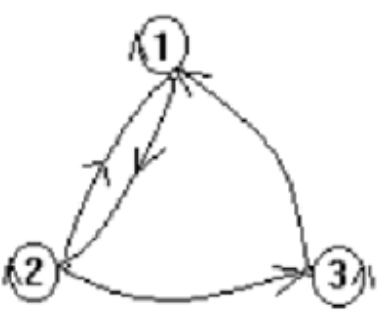
\includegraphics[width=0.2\linewidth]{figure/2-1-1}
	\caption{习题2-1-1图}
	\label{fig:2-1-1}
\end{figure}


则 $R$ 具有(\qquad)性质.
\begin{choices}
	\item 自反性
	\item 反自反性、反对称性、传递性
	\item 反自反性、反对称性
	\item 自反性、对称性、传递性
\end{choices}

\item 设 $|A|=n$,则 $A$ 上有(\quad)二元关系.
\begin{choices}
	\item $2^n$
	\item $2^{n^2}$
	\item $n^2$
	\item $n^n$
\end{choices}

\item  设 \(A=\{\varnothing,\{1\},\{1,3\},\{1,2,3\}\}\),则 \(A\) 上包含关系“\(\subseteq\)”的哈斯图为(\quad).
\begin{choices}
	\item
	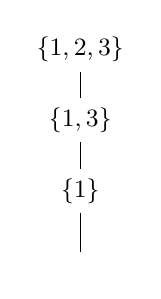
\begin{tikzpicture}[scale=0.9, every node/.style={font=\small}]
		\node (t) at (0,3) {\(\{1,2,3\}\)};
		\node (m2) at (0,2) {\(\{1,3\}\)};
		\node (m1) at (0,1) {\(\{1\}\)};
		\node (b) at (0,0) {\(\varnothing\)};
		\draw (t)--(m2)--(m1)--(b);
	\end{tikzpicture}
	\item
	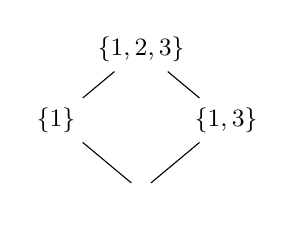
\begin{tikzpicture}[scale=0.9, every node/.style={font=\small}]
		\node (t) at (0,2) {\(\{1,2,3\}\)};
		\node (l) at (-1.2,1) {\(\{1\}\)};
		\node (r) at (1.2,1) {\(\{1,3\}\)};
		\node (b) at (0,0) {\(\varnothing\)};
		\draw (t)--(l)--(b)--(r)--(t);
	\end{tikzpicture}
	
	\item
	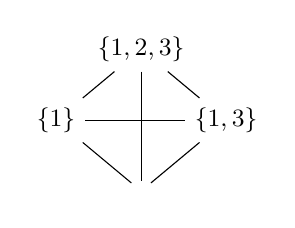
\begin{tikzpicture}[scale=0.9, every node/.style={font=\small}]
		\node (t) at (0,2) {\(\{1,2,3\}\)};
		\node (l) at (-1.2,1) {\(\{1\}\)};
		\node (r) at (1.2,1) {\(\{1,3\}\)};
		\node (b) at (0,0) {\(\varnothing\)};
		\draw (t)--(l)--(b)--(r)--(t);
		\draw (l)--(r);
		\draw (t)--(b);
	\end{tikzpicture}
	
	\item
	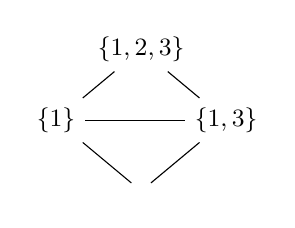
\begin{tikzpicture}[scale=0.9, every node/.style={font=\small}]
		\node (t) at (0,2) {\(\{1,2,3\}\)};
		\node (l) at (-1.2,1) {\(\{1\}\)};
		\node (r) at (1.2,1) {\(\{1,3\}\)};
		\node (b) at (0,0) {\(\varnothing\)};
		\draw (t)--(l)--(b)--(r)--(t);
		\draw (l)--(r);
	\end{tikzpicture}
\end{choices}

\item 下列关系,(\quad)能构成函数.
\begin{choices}
	\item \( f=\left\{\langle x_1,x_2\rangle \mid x_1,x_2\in\mathbb{R},\,x_1=x_2^2\right\}\)
	\item \( f=\left\{\langle x_1,x_2\rangle \mid (x_1,x_2\in\mathbb{N} )\land (x_1+x_2=10)\right\}\)
	\item \( f=\left\{\langle x,\lvert x\rvert\rangle \mid x\in\mathbb{R}\right\}\)
	\item \( f=\left\{\langle x_1,x_2\rangle \mid x_1,x_2\in\mathbb{N},\,x_2\text{为小于}x_1\text{的素数的个数}\right\}\)
\end{choices}

\item 设 $S=\{1,2,3\}$,$R$ 为 $S$ 上的关系,其关系图为:元素 $1,2,3$ 各有一个自环.

\begin{figure}[H]
	\centering
	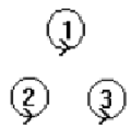
\includegraphics[width=0.2\linewidth]{figure/2-1-5}
	\caption{习题2-1-5图}
	\label{fig:2-1-5}
\end{figure}


则 $R$ 具有(\quad) 的性质.
\begin{choices}
	\item 反自反、反对称、传递
	\item 自反、对称、传递
	\item 什么性质也没有
	\item 自反、对称、反对称、传递
\end{choices}


\item 设 $A=\{1,2,3\}$,则 $A$ 上有(\quad)个二元关系.

\begin{choices}
	\item $2^{3^2}$
	\item $2^3$
	\item $2^{2^3}$
	\item $3^2$
\end{choices}


\item 设 \(R,\,S\) 是集合 \(A\) 上的关系,则下列(\quad)断言是正确的.
\begin{choices}
	\item 若 \(R,\,S\) 传递的,则 \(R\circ S\) 是传递的
	\item 若 \(R,\,S\) 反对称的,则 \(R\circ S\) 是反对称的
	\item 若 \(R,\,S\) 对称的,则 \(R\circ S\) 是对称的
	\item \(R,\,S\) 自反的,则 \(R\circ S\) 是自反的
\end{choices}


\item 集合 \(A=\{1,2,3,4\}\) 上的偏序关系图为(如题图所示),则它的哈斯图为(\qquad).

\begin{figure}[H]
	\centering
	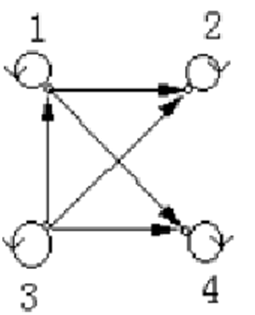
\includegraphics[width=0.2\linewidth]{figure/2-1-8}
	\caption{习题2-1-8图}
	\label{fig:2-1-8}
\end{figure}

\begin{choices}
	\item
	\begin{tikzpicture}[scale=0.9, every node/.style={font=\small}]
		\node (1) at (0,0) {1};
		\node (2) at (-0.9,1.0) {2};
		\node (4) at (0.9,1.0) {4};
		\node (3) at (0,-1.2) {3};
		\draw (1)--(2);
		\draw (1)--(4);
		\draw (1)--(3);
	\end{tikzpicture}
	
	\item
	\begin{tikzpicture}[scale=0.9, every node/.style={font=\small}]
		\node (1) at (-1.0,1.0) {1};
		\node (3) at (-0.3,0.0) {3};
		\node (4) at (0,-0.8) {4};
		\node (2) at (1.0,0.2) {2};
		\draw (1)--(3)--(4)--(2);
	\end{tikzpicture}
	
	\item
	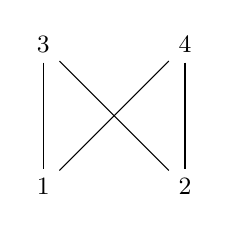
\begin{tikzpicture}[scale=0.9, every node/.style={font=\small}]
		\node (3) at (-1,1) {3};
		\node (1) at (-1,-1) {1};
		\node (4) at (1,1) {4};
		\node (2) at (1,-1) {2};
		\draw (3)--(1);
		\draw (4)--(2);
		\draw (3)--(2);
		\draw (1)--(4);
	\end{tikzpicture}
	
	\item
	\begin{tikzpicture}[scale=0.9, every node/.style={font=\small}]
		\node (2) at (0,1.5) {2};
		\node (4) at (0,0.5) {4};
		\node (1) at (0,-0.5) {1};
		\node (3) at (0,-1.5) {3};
		\draw (2)--(4)--(1)--(3);
	\end{tikzpicture}
\end{choices}


\item 设集合 $A=\{1,2,3,4,5\}$ 上偏序关系的 Hasse 图为

\begin{center}
	\begin{tikzpicture}[scale=1.0]
		\node[circle,draw,inner sep=1.2pt,label=above:{\small 1}] (n1) at (0,2) {};
		\node[circle,draw,inner sep=1.2pt,label=left:{\small 2}] (n2) at (-1,1) {};
		\node[circle,draw,inner sep=1.2pt,label=right:{\small 3}] (n3) at (1,1) {};
		\node[circle,draw,inner sep=1.2pt,label=below:{\small 4}] (n4) at (0,0) {};
		\node[circle,draw,inner sep=1.2pt,label=right:{\small 5}] (n5) at (2,-0.5) {};
		
		\draw (n1)--(n2);
		\draw (n1)--(n3);
		\draw (n2)--(n4);
		\draw (n4)--(n3);
		\draw (n3)--(n5);
	\end{tikzpicture}
\end{center}

求:子集 $B=\{2,3,4\}$ 的最大元(\quad);最小元(\quad);极大元(\quad);
极小元(\quad);\\上界(\quad);上确界(\quad);下界(\quad);下确界(\quad).

\begin{choices}
	\item 无,4,5,2,3,4,5,1,1,4,4
	\item 无,4,2,3,4,5,1,1,4,4
	\item 无,4,2,3,4,1,1,4,无
	\item 无,4,2,3,4,1,1,4,4
\end{choices}


\item 设 \(A=\{1,2,3,4,5,6\}\),\(B=\{1,2,3\}\),从 \(A\) 到 \(B\) 的关系
\(R=\{\langle x,y\rangle \mid x=y^2\}\),\(R=\underline{\hspace{2cm}}\);\(R^{-1}=\underline{\hspace{2cm}}\).

\item 设 $A=\{1,2,3,4,5,6\}$,$R$ 是 $A$ 上的整除关系,求 $R=\{(\qquad\qquad)\}$.


\item 设 \(A=\{1,2,3,4,5,6\}\),\(B=\{1,2,3\}\),从 \(A\) 到 \(B\) 的关系
\(R=\{\langle x,y\rangle \mid x=2y\}\),\(R=\underline{\hspace{2cm}}\);\(R^{-1}=\underline{\hspace{2cm}}\).


\item 设 $A=\{a,b,c\}$,$A$ 上二元关系
$R=\{\langle a,a\rangle,\langle a,b\rangle,\langle a,c\rangle,\langle c,c\rangle\}$.

则 $s(R)=$ \underline{\hspace{2cm}}.


\item 设 $A=\{a,b,c,d\}$,其上偏序关系 $R$ 的哈斯图为
\begin{center}
	\begin{tikzpicture}[scale=1]
		\node (d) at (0,2) {$d$};
		\node (b) at (-1,1) {$b$};
		\node (c) at (1,1) {$c$};
		\node (a) at (0,0) {$a$};
		\draw (a) -- (b) -- (d) -- (c) -- (a);
	\end{tikzpicture}
\end{center}
则 $R=\underline{\hspace{2cm}}$.


\item 集合A上的偏序关系的三个性质是\underline{\hspace{2cm}}.

\item 设 $A=\{1,2,3,4\}$,$A$ 上关系图为:
\begin{center}
	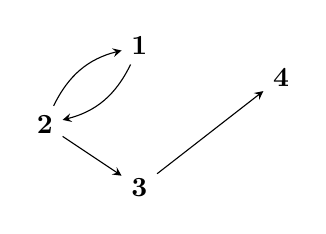
\begin{tikzpicture}[>=stealth, node distance=2cm]
		\node (1) at (0,1.8) {\textbf{1}};
		\node (2) at (-1.2,0.8) {\textbf{2}};
		\node (3) at (0,0) {\textbf{3}};
		\node (4) at (1.8,1.4) {\textbf{4}};
		\draw[->] (2) to[bend left=25] (1);
		\draw[->] (1) to[bend left=25] (2);
		\draw[->] (2) -- (3);
		\draw[->] (3) -- (4);
	\end{tikzpicture}
\end{center}
则 $R^2=\underline{\hspace{2cm}}$.

\item 举出集合A上的既是等价关系又是偏序关系的一个例子\underline{\hspace{2cm}}.

\item 设 $A=\{1,2,3,4,5,6\}$,$B=\{1,2,3\}$,从 $A$ 到 $B$ 的关系 $R=\{(x,y)\mid x=y^2\}$,
求 $R$ 和 $R^{-1}$ 的关系矩阵.


\item 集合A上的等价关系的三个性质是\underline{\hspace{2cm}}.


\item 设 $S=\{1,2,3,4\}$,$A$ 上的关系
$R=\{\langle 1,2\rangle,\langle 2,1\rangle,\langle 2,3\rangle,\langle 3,4\rangle\}$.
求:
\begin{enumerate}
	\item $R\circ R$
	\item $R^{-1}$
\end{enumerate}


\end{enumerate}
\newpage

\section{第三章测试题}

\begin{enumerate}
	\item 永真式的否定是(\quad).
	\begin{choices}
		\item (B)--(D)均有可能
		\item 永真式
		\item 可满足式
		\item 永假式
	\end{choices}
	
	\item 命题逻辑演绎的 CP 规则为(\quad).
	\begin{choices}
		\item 在推演过程中可随便使用前提
		\item 在推演过程中可随便使用前面演绎出的某些公式的逻辑结果
		\item 设 $\Phi(A)$ 是含公式 $A$ 的命题公式,$B \Leftrightarrow A$,则可用 $B$ 替换 $\Phi(A)$ 中的 $A$
		\item 如果要演绎出的公式为 $B \to C$ 形式,那么将 $B$ 作为前提,设法演绎出 $C$
	\end{choices}
	
	\item $\neg (p \wedge q) \to r$ 的主析取范式中含极小项的个数为(\quad).
	\begin{choices}
		\item 3
		\item 0
		\item 5
		\item 2
	\end{choices}
	
	\item 下列语句是命题的有(\quad).
	\begin{choices}
		\item 我正在说谎
		\item $x+y>0$
		\item $xy>0$ 且仅当 $x$ 和 $y$ 都大于 0
		\item 明年中秋节的晚上是晴天
	\end{choices}
	
	\item 下列符号串是合式公式的有(\quad).
	\begin{choices}
		\item $P \Leftrightarrow Q$
		\item $P \Rightarrow P \vee Q$
		\item $\neg (P \Leftrightarrow Q)$
		\item $(\neg P \vee Q)\wedge (P \vee \neg Q)$
	\end{choices}
	
	\item 下列哪些公式为永真蕴含式？(\quad)
	\begin{choices}
		\item $\neg Q \Rightarrow P \to Q$
		\item $\neg Q \Rightarrow Q \to P$
		\item $\neg P \wedge (P \vee Q) \Rightarrow \neg P$
		\item $P \Rightarrow P \to Q$
	\end{choices}
	
	\item 全体小项合取式为(\quad).
	\begin{choices}
		\item $A,B,C$ 都有可能
		\item 矛盾式
		\item 永真式
		\item 可满足式
	\end{choices}
	
	\item 下列公式是重言式的有(\quad).
	\begin{choices}
		\item $\neg (Q \to P)\wedge P$
		\item $(P \wedge Q)\to Q$
		\item $\neg (P \Leftrightarrow Q)$
		\item $(P \to Q)\Leftrightarrow P$
	\end{choices}
	
	\item 下列等价式成立的有(\quad).
	\begin{choices}
		\item $P \wedge (P \to Q)\Leftrightarrow Q$
		\item $P \to (Q \to R)\Leftrightarrow (P \wedge Q)\to R$
		\item $P \vee (P \wedge R)\Leftrightarrow R$
		\item $P \to Q \Leftrightarrow \neg Q \to \neg P$
	\end{choices}
	
	\item $(P \to Q)\to R$ 的合取范式为(\quad).
	\begin{choices}
		\item $(P \vee Q \vee R)\wedge (P \vee \neg Q \vee R)\wedge (P \vee \neg Q \vee R)\wedge (\neg P \vee \neg Q \vee R)$
		\item $(P \vee R)\wedge (\neg Q \vee R)$
		\item $(P \wedge \neg Q)\vee R$
		\item $(P \wedge \neg Q \wedge R)\vee (P \wedge \neg Q \wedge \neg R)\vee (P \wedge Q \wedge R)\vee (P \wedge \neg Q \wedge R)\vee (\neg P \wedge Q \wedge R)\vee (\neg P \wedge \neg Q \wedge R)$
	\end{choices}
	
	\item 下列等价式成立的有(\quad).
	\begin{choices}
		\item $P \vee (P \wedge R)\Leftrightarrow R$
		\item $P \to Q \Leftrightarrow \neg Q \to \neg P$
		\item $P \to (Q \to R)\Leftrightarrow (P \wedge Q)\to R$
		\item $P \wedge (P \to Q)\Leftrightarrow Q$
	\end{choices}
	
	\item 下列各命题中真值为真的命题有(\quad).
	\begin{choices}
		\item $2+2=4$ 当且仅当 $3$ 是奇数
		\item $2+2\neq 4$ 当且仅当 $3$ 是奇数
		\item $2+2\neq 4$ 当且仅当 $3$ 不是奇数
		\item $2+2=4$ 当且仅当 $3$ 不是奇数
	\end{choices}
	
	\item 下列语句是命题的有(\quad).
	\begin{choices}
		\item $xy>0$ 且仅当 $x$ 和 $y$ 都大于 0
		\item 我正在说谎
		\item 明年中秋节的晚上是晴天
		\item $x+y>0$
	\end{choices}
	
	\item 下列哪些是简单命题？
	\begin{choices}
		\item 中国有四大发明
		\item 3 是素数或者 4 是素数
		\item 刘红与赵欣是同学
		\item 你去图书馆吗
	\end{choices}
	
	\item 下列公式中哪些是永真式？(\quad)
	\begin{choices}
		\item $(\neg P \wedge Q)\to (Q\to \neg R)$
		\item $(P \wedge Q)\to P$
		\item $P\to (P\vee Q)$
		\item $P\to (Q\to Q)$
	\end{choices}
	
	\item $A,B$ 为二合式公式,且 $A \Leftrightarrow B$,则(\quad).
	\begin{choices}
		\item $A \Leftrightarrow B$ 为重言式
		\item $A \to B$ 为重言式
		\item $A' \Leftrightarrow B'$
		\item $A' \Rightarrow B'$
		\item $A \Rightarrow B$
	\end{choices}
	
	\item 判断下列语句是不是命题.若是,给出命题的真值(\quad).
	\begin{choices}
		\item 北京是中华人民共和国的首都
		\item 若 $7+8>18$,则三角形有 4 条边
		\item 给我一杯水吧
		\item 前进
		\item 你喜欢唱歌吗
		\item 陕西师大是一座工厂
	\end{choices}
	
	\item 下列问题成立的有(\quad).
	\begin{choices}
		\item 若 $A \wedge C \Leftrightarrow B \wedge C$,则 $A \Leftrightarrow B$
		\item 若 $A \vee C \Leftrightarrow B \vee C$,则 $A \Leftrightarrow B$
		\item 若 $\neg A \Leftrightarrow \neg B$,则 $A \Leftrightarrow B$
		\item 若 $A \Leftrightarrow B$,则 $\neg A \Leftrightarrow \neg B$
	\end{choices}
	
	\item 下列语句不是命题的有(\quad).
	\begin{choices}
		\item $x=13$
		\item 你打算考硕士研究生吗
		\item 鸡有三只脚
		\item 离散数学是计算机系的一门必修课
		\item 太阳系以外的星球上有生物
	\end{choices}
	
	\item \underline{\hspace{2cm}}称为命题.
	
	\item 设 \textbf{P}：我生病,\textbf{Q}：我去学校,则下列命题可符号化为：
	
	\begin{enumerate}
		\item[(1)] 只有在生病时,我才不去学校
		\item[(2)] 若我生病,则我不去学校
		\item[(3)] 当且仅当我生病时,我才不去学校
		\item[(4)] 若我不生病,则我一定去学校
	\end{enumerate}
	
	\item $\neg((P\land Q)\lor R)\to R$ 的主合取范式为 \underline{\hspace{2cm}}.
	
	\item 所有小项的析取式为 \underline{\hspace{2cm}}.
	
	\item 命题“$2$是偶数或$-3$是负数”的否定是( \ \ ).
	
	\item 公式 $(P\land R)\lor(S\land R)\lor\neg P$ 的主合取范式为 \underline{\hspace{2cm}}.
	
	\item $\sqrt{2}$ 是有理数的真值为 \underline{\hspace{2cm}}.
	
	\item \textbf{Q}：我将去上海,\textbf{R}：我有时间,公式 $(Q\to R)\land(R\to Q)$ 的自然语言为：\underline{\hspace{2cm}}.
	
	\item \textbf{P}、\textbf{Q}真值为$0$;\textbf{R}、\textbf{S}真值为$1$.则公式 $\bigl(P\land(R\lor S)\to((P\lor Q)\land(R\land S))\bigr)$ 的真值为 \underline{\hspace{2cm}}.
	
	\item \textbf{P}：你努力,\textbf{Q}：你失败.“除非你努力,否则你将失败”的翻译为 \underline{\hspace{2cm}},“虽然你努力了,但还是失败了”的翻译为 \underline{\hspace{2cm}}.
	
	\item 公式 $(\neg P\land Q)\lor(\neg P\land \neg Q)$ 化简为( \ \ ),公式 $Q\to(P\lor(P\land Q))$ 可化简为( \ \ ).
	
	\item 一个命题含有 $4$ 个原子命题,则对其所有可能赋值有 \underline{\hspace{2cm}} 种.
	
	\item 命题 $P\to Q$ 的真值为$0$,当且仅当 \underline{\hspace{2cm}}.
	
	\item 设 \textbf{P}、\textbf{Q} 的真值为$0$,\textbf{R}、\textbf{S} 的真值为$1$,则 $\neg\bigl(P\lor(Q\to(R\land \neg P))\bigr)\to(R\lor \neg S)$ 的真值 $=$ \underline{\hspace{2cm}}.
\end{enumerate}

\newpage

\section{第四章测试题}

\begin{enumerate}
	\item 公式 \(A=\exists x(P(x)\to Q(x))\) 的解释 \(I\) 为：个体域 \(D=\{2\}\),\(P(x):x>3\),\(Q(x):x=4\),则 \(A\) 的真值为(\quad).
	\begin{choices}
		\item 无法判定
		\item 可满足式
		\item \(1\)
		\item \(0\)
	\end{choices}
	
	\item 命题“有的人喜欢所有的花”的逻辑符号化为(\quad).
	
	设 \(D\)：全总个体域,\(F(x)\)：\(x\) 是花,\(M(x)\)：\(x\) 是人,\(H(x,y)\)：\(x\) 喜欢 \(y\).
	\begin{choices}
		\item \(\forall x\bigl(M(x)\to \forall y(F(y)\to H(x,y))\bigr)\)
		\item \(\exists x\bigl(M(x)\to \forall y(F(y)\to H(x,y))\bigr)\)
		\item \(\forall x\bigl(M(x)\land \forall y(F(y)\to H(x,y))\bigr)\)
		\item \(\exists x\bigl(M(x)\land \forall y(F(y)\to H(x,y))\bigr)\)
	\end{choices}
	
	\item 下列等价关系正确的是(\quad).
	\begin{choices}
		\item \(\neg \forall x(P(x)\vee Q(x))\Leftrightarrow \neg \forall xP(x)\vee \neg \forall xQ(x)\)
		\item \(\forall x(P(x)\to Q)\Leftrightarrow \forall xP(x)\to Q\)
		\item \(\exists x(P(x)\vee Q(x))\Leftrightarrow \exists xP(x)\vee \exists xQ(x)\)
		\item \(\exists x(P(x)\to Q)\Leftrightarrow \exists xP(x)\to Q\)
	\end{choices}
	
	\item “人总是要死的”谓词公式表示为(\quad).
	
	(论域为全总个体域)\(M(x)\)：\(x\) 是人;\(\operatorname{Mortal}(x)\)：\(x\) 是要死的.
	\begin{choices}
		\item \(\exists x\bigl(M(x)\land \operatorname{Mortal}(x)\bigr)\)
		\item \(\forall x\bigl(M(x)\to \operatorname{Mortal}(x)\bigr)\)
		\item \(M(x)\land \operatorname{Mortal}(x)\)
		\item \(M(x)\to \operatorname{Mortal}(x)\)
	\end{choices}
	
	\item 下列推导错在(\quad).
	
	\begin{tabular}{lll}
		\textcircled{1} & \(\forall x\exists y(x>y)\) & \(P\) \\
		\textcircled{2} & \(\exists y(z>y)\) & \(US\)\textcircled{1} \\
		\textcircled{3} & \((z>C_z)\) & \(ES\)\textcircled{2} \\
		\textcircled{4} & \(\forall x(x>x)\) & \(UG\)\textcircled{3}
	\end{tabular}
	\begin{choices}
		\item \textcircled{4}
		\item \textcircled{3}
		\item 无
		\item \textcircled{2}
	\end{choices}
	
	\item 给定推理
	
	\begin{tabular}{lll}
		\textcircled{1} & \(\forall x(F(x)\to G(x))\) & \(P\) \\
		\textcircled{2} & \(F(y)\to G(y)\) & \(US\)\textcircled{1} \\
		\textcircled{3} & \(\exists xF(x)\) & \(P\) \\
		\textcircled{4} & \(F(y)\) & \(ES\)\textcircled{3} \\
		\textcircled{5} & \(G(y)\) & \(T\)\textcircled{2}\textcircled{4}\(I\) \\
		\textcircled{6} & \(\forall xG(x)\) & \(UG\)\textcircled{5}
	\end{tabular}
	
	\(\therefore\ \forall x(F(x)\to G(x))\land \exists xF(x)\Rightarrow \forall xG(x)\)
	
	推理过程中错在(\quad).
	\begin{choices}
		\item \textcircled{1}\(\to\)\textcircled{2}
		\item \textcircled{4}\(\to\)\textcircled{5}
		\item \textcircled{5}\(\to\)\textcircled{6}
		\item \textcircled{3}\(\to\)\textcircled{4}
		\item \textcircled{2}\(\to\)\textcircled{3}
	\end{choices}
	
	\item 公式 \(\forall x\forall y(P(x,y)\vee Q(y,z))\land \exists xP(x,y)\) 换名(\quad).
	\begin{choices}
		\item \(\forall x\forall y(P(x,u)\vee Q(u,z))\land \exists xP(x,u)\)
		\item \(\forall u\forall y(P(u,y)\vee Q(y,z))\land \exists uP(u,y)\)
		\item \(\forall x\forall u(P(x,u)\vee Q(u,z))\land \exists xP(x,y)\)
		\item \(\forall x\forall y(P(x,y)\vee Q(y,z))\land \exists xP(x,u)\)
	\end{choices}
	
	\item 下列推理步骤错在(\quad).
	
	\begin{tabular}{lll}
		\textcircled{1} & \(\forall x\exists yF(x,y)\) & \(P\) \\
		\textcircled{2} & \(\exists yF(z,y)\) & \(US\)\textcircled{1} \\
		\textcircled{3} & \(F(z,c)\) & \(ES\)\textcircled{2} \\
		\textcircled{4} & \(\forall xF(x,c)\) & \(UG\)\textcircled{3} \\
		\textcircled{5} & \(\exists y\forall xF(x,y)\) & \(EG\)\textcircled{4}
	\end{tabular}
	\begin{choices}
		\item \textcircled{2}\(\to\)\textcircled{3}
		\item \textcircled{4}\(\to\)\textcircled{5}
		\item \textcircled{3}\(\to\)\textcircled{4}
		\item \textcircled{1}\(\to\)\textcircled{2}
	\end{choices}
	
	\item “没有不犯错误的人”的逻辑符号化为(\quad).
	
	设 \(H(x)\)：\(x\) 是人,\(P(x)\)：\(x\) 犯错误.
	\begin{choices}
		\item \(\forall x(H(x)\to P(x))\)
		\item \(\exists x(H(x)\to P(x))\)
		\item \(\neg(\exists x(H(x)\to \neg P(x)))\)
		\item \(\neg(\exists x(H(x)\land \neg P(x)))\)
	\end{choices}
	
	\item 下面蕴涵关系成立的是(\quad).
	\begin{choices}
		\item \(\exists x\forall yA(x,y)\Rightarrow \forall y\exists xA(x,y)\)
		\item \(\forall xP(x)\land \forall xQ(x)\Rightarrow \forall x(P(x)\vee Q(x))\)
		\item \(\forall xP(x)\to \forall xQ(x)\Rightarrow \forall x(P(x)\to Q(x))\)
		\item \(\exists xP(x)\to \forall xQ(x)\Rightarrow \forall x(P(x)\to Q(x))\)
	\end{choices}
	
	\item 给定公式 \(\exists xP(x)\to \forall xP(x)\),当 \(D=\{a,b\}\) 时,解释(\quad)使该公式真值为 \(0\).
	\begin{choices}
		\item \(P(a)=1,\ P(b)=0\)
		\item \(P(a)=0,\ P(b)=1\)
		\item \(P(a)=1,\ P(b)=1\)
		\item \(P(a)=0,\ P(b)=0\)
	\end{choices}

	
	\item 命题“对于任意给定的正实数,都存在比它大的实数”令 \(F(x)\)：\(x\) 为正实数,\(L(x,y):x>y\),则命题的逻辑谓词公式为 \underline{\hspace{2cm}}.
	
	\item 设谓词 \(P(x)\)：\(x\) 是奇数,\(Q(x)\)：\(x\) 是偶数,谓词公式 \(\exists x(P(x)\vee Q(x))\) 在哪个个体域中为真？(\quad)
	\begin{choices}
		\item 自然数
		\item 实数
		\item 复数
		\item 以上均成立
	\end{choices}
	
	\item 公式 \((\forall y(P(x,y)\land \exists zQ(x,z))\vee \forall xR(x,y))\) 中的自由变元为 \underline{\hspace{2cm}}.
	
	\item 若解释 \(I\) 的论域 \(D\) 仅包含一个元素,则 \(\exists xP(x)\to \forall xP(x)\) 在 \(I\) 下真值为 \underline{\hspace{2cm}}.
	
	\item 设 \(x\) 是谓词合式公式 \(A\) 的一个客体变元,\(A\) 的论域为 \(D\),\(A(x)\) 关于 \(y\) 是自由的,则 \underline{\hspace{2cm}} 被称为存在量词消去规则,记为 \(ES\).
	
	\item 令 \(R(x)\)：\(x\) 是实数,\(Q(x)\)：\(x\) 是有理数.则命题“并非每个实数都是有理数”的符号化表示为(\quad).
	
	\underline{\hspace{2cm}}
	
	\item 公式 \(\forall x(A(x)\to B(y,x))\land \exists zC(y,z)\to D(x)\) 中,自由变元是(\quad),约束变元是(\quad).
	
	\underline{\hspace{2cm}}
	
	\underline{\hspace{2cm}}
	
	\item 令 \(E(x)\)：\(x\) 是偶数,\(D(x,y)\)：\(x\) 除尽 \(y\).则 \(\forall x(E(x)\to \forall y(D(x,y)\to E(y)))\) 的汉语翻译为
	
	\underline{\hspace{2cm}}
	
	\item 谓词合式公式 \(\forall xP(x)\to \exists xQ(x)\) 的前束范式为 \underline{\hspace{2cm}}.
	
	\item 设全体域 \(D\) 是正整数集合,确定下列命题的真值：
	
	\begin{tabular}{ll}
		\((1)\ \forall x\exists y(xy=y)\) & (\quad) \\
		\((2)\ \exists x\forall y(x+y=y)\) & (\quad) \\
		\((3)\ \exists x\forall y(x+y=x)\) & (\quad) \\
		\((4)\ \forall x\exists y(y=2x)\) & (\quad)
	\end{tabular}
	
	\underline{\hspace{2cm}}
	
	\underline{\hspace{2cm}}
	
	\underline{\hspace{2cm}}
	
	\underline{\hspace{2cm}}
	
	\item 谓词公式 \(\forall x\forall y(\exists z(P(x,z)\land P(y,z))\to \exists uQ(x,y,u))\) 的前束范式为
	
	\underline{\hspace{2cm}}
	
	\item 论域 \(D=\{1,2\}\),指定谓词 \(P\) 如下：
	
	\begin{center}
		\begin{tabular}{c|cccc}
			& \(P(1,1)\) & \(P(1,2)\) & \(P(2,1)\) & \(P(2,2)\) \\
			\hline
			& \(T\) & \(T\) & \(F\) & \(F\)
		\end{tabular}
	\end{center}
	
	则公式 \(\forall x\exists yP(y,x)\) 真值为 \underline{\hspace{2cm}}.
	
	\item 设 \(x\) 是谓词合式公式 \(A\) 的一个客体变元,\(A\) 的论域为 \(D\),\(A(x)\) 关于 \(y\) 自由的,则 \underline{\hspace{2cm}} 被称为全称量词消去规则,记为 \(US\).
	
	\item \(\forall xF(x)\land \neg(\exists xG(x))\) 的前束范式为 \underline{\hspace{2cm}}.
	
	\item 谓词公式 \(\forall x(P(x)\vee \exists yR(y))\to Q(x)\) 中量词 \(\forall x\) 的辖域是(\quad).
	
	\underline{\hspace{2cm}}
	
	\item 设 \(P(x)\)：\(x\) 是素数,\(O(x)\)：\(x\) 是奇数,\(N(x,y)\)：\(x\) 可以整除 \(y\).则谓词公式 \(\forall x(P(x)\to \exists y(O(y)\land N(y,x)))\) 的自然语言是
	
	\underline{\hspace{2cm}}
\end{enumerate}

